\documentclass[12pt]{beamer}

% \usepackage{cmap}
\usepackage[english, russian]{babel}

\usetheme{metropolis}
\usepackage{appendixnumberbeamer}

\usepackage{booktabs}
\usepackage{minted}
\usepackage[many]{tcolorbox}
\usepackage{mdframed}

\usepackage{listings}
\lstset{basicstyle=\ttfamily\small,
	showstringspaces=false,
	breaklines=true,
	frame=lrtb,
	% numbers=left,
	extendedchars=\true,
	language=Java
}

\usepackage{xcolor}

\usepackage{xspace}
\newcommand{\themename}{\textbf{\textsc{metropolis}}\xspace}
% \setsansfont{Fira Sans Bold}

% \surroundwithmdframed{minted}

\title{Автоматизация миграции программного кода на новый набор библиотек}
% \subtitle{A modern beamer theme}
\date{\today}
\author[Алексюк Артем]{
    Студент: Алексюк Артем\\
    гр. 63501/3\\ \\
    Руководитель: Ицыксон В.М.\\
    Аттестация №2
}

\newtcolorbox{mybox}[1][]{
    width=\textwidth,
    arc=3mm,
%    auto outer arc,
    boxsep=0cm,
    toprule=1pt,
    leftrule=1pt,
    bottomrule=1pt,
    rightrule=1pt,
    colframe=white,
    boxrule=0pt,frame hidden,
    breakable,
    nobeforeafter,
    enhanced jigsaw,
    opacityframe=0.7,
    fontupper=\bfseries,
    opacityback=0.7
}

\setbeamercolor{itemize/enumerate body}{fg=black}

% \setbeamertemplate{blocks}[rounded][shadow=false]
% \addtobeamertemplate{block begin}{\pgfsetfillopacity{0.5}}{\pgfsetfillopacity{1}}

\begin{document}

\maketitle

%\begin{frame}{Table of contents}
%  \setbeamertemplate{section in toc}[sections numbered]
%  \tableofcontents[hideallsubsections]
%\end{frame}

% \section{Introduction}


{
\usebackgroundtemplate{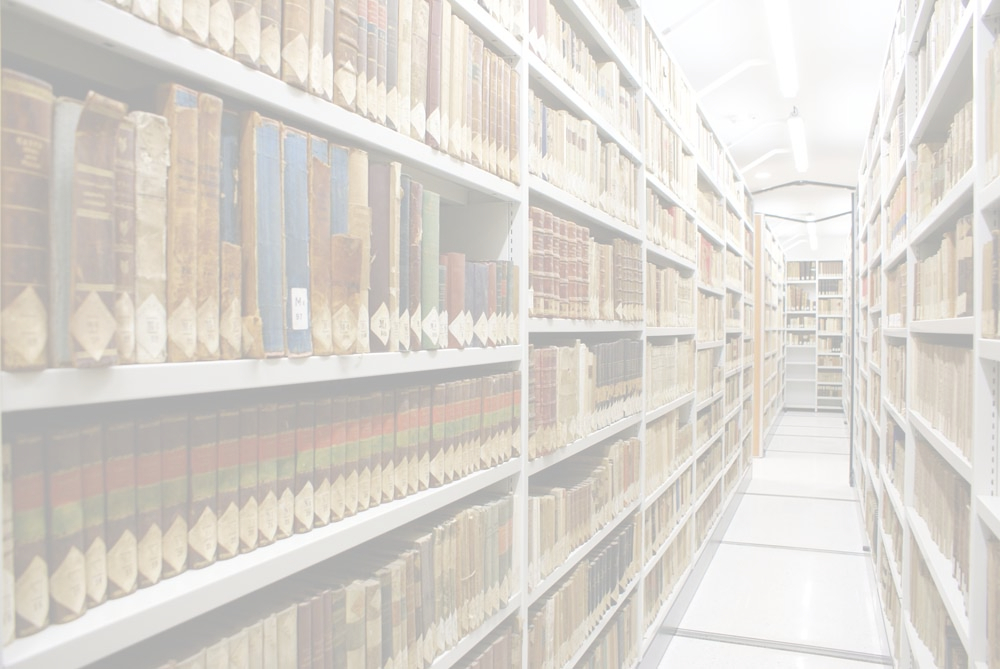
\includegraphics[height=\paperheight,width=\paperwidth]{historical-archive.jpg};}
\begin{frame}{Актуальность}
\begin{mybox}[]
Миграция (портирование) в новое библиотечное окружение:
\begin{itemize}
	\item Новая программная платформа
	\item Новая аппаратная платформа
	\item Новая версия библиотеки
	\item Унаследованный (несовместимый) код 
	\item ...		
\end{itemize}
\end{mybox}
\end{frame}
}

\begin{frame}[fragile]{Пример задачи миграции}
	Программа, использующая библиотеку java.net.URLConnection:
\begin{minted}[breaklines,fontsize=\small]{java}
URL url = new URL("http://api.ipify.org/");
URLConnection conn = url.openConnection();
\end{minted}
	Программа, использующая библиотеку Apache HttpClient:
\begin{minted}[breaklines,fontsize=\small]{java}
CloseableHttpClient httpclient = HttpClients.createDefault();
HttpGet httpget = new HttpGet("http://api.ipify.org/");
CloseableHttpResponse httpResponse = httpclient.execute(httpget);
\end{minted}
\end{frame}

\begin{frame}{Общая схема решения задачи}
\begin{center}
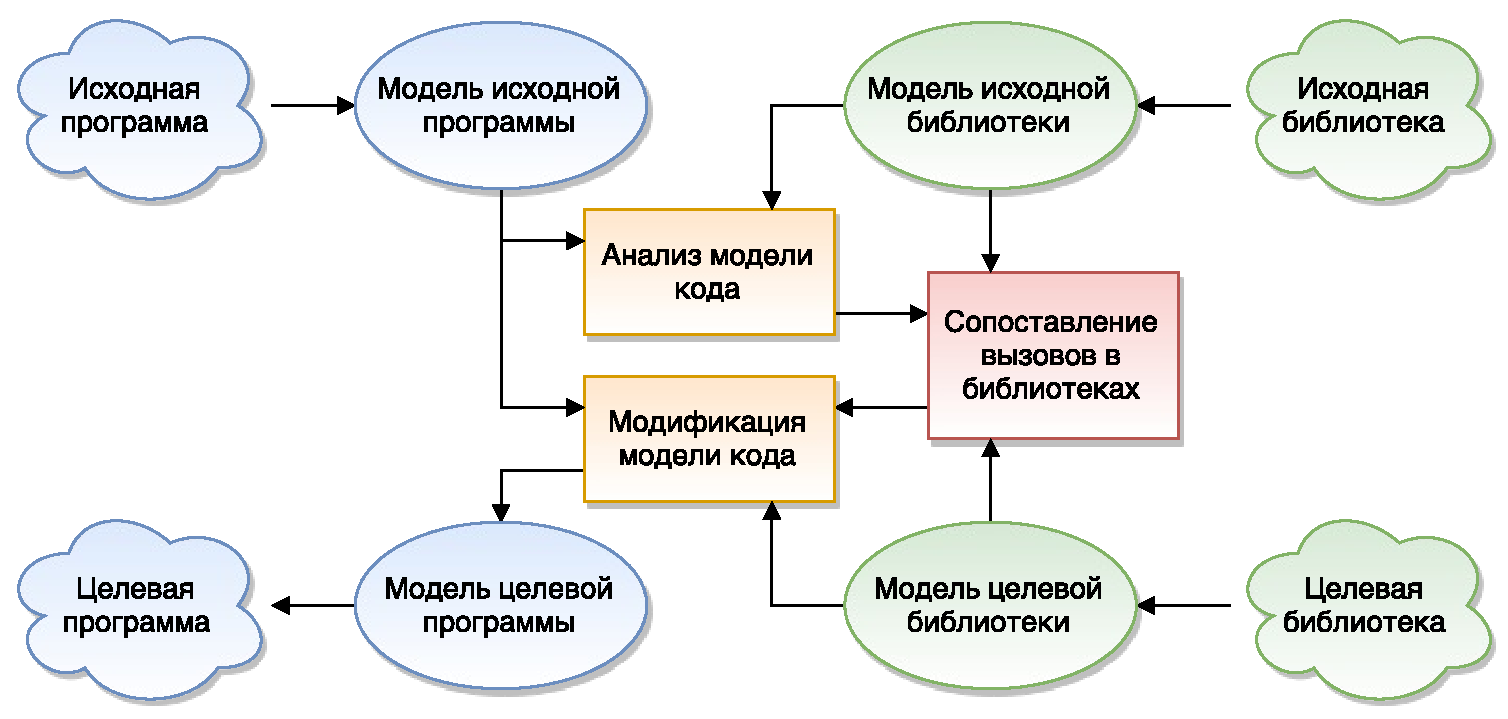
\includegraphics[width=\textwidth]{scheme.pdf}
\end{center}
\end{frame}

\begin{frame}{Фрагмент модели библиотеки URLConnection}
\begin{center}
	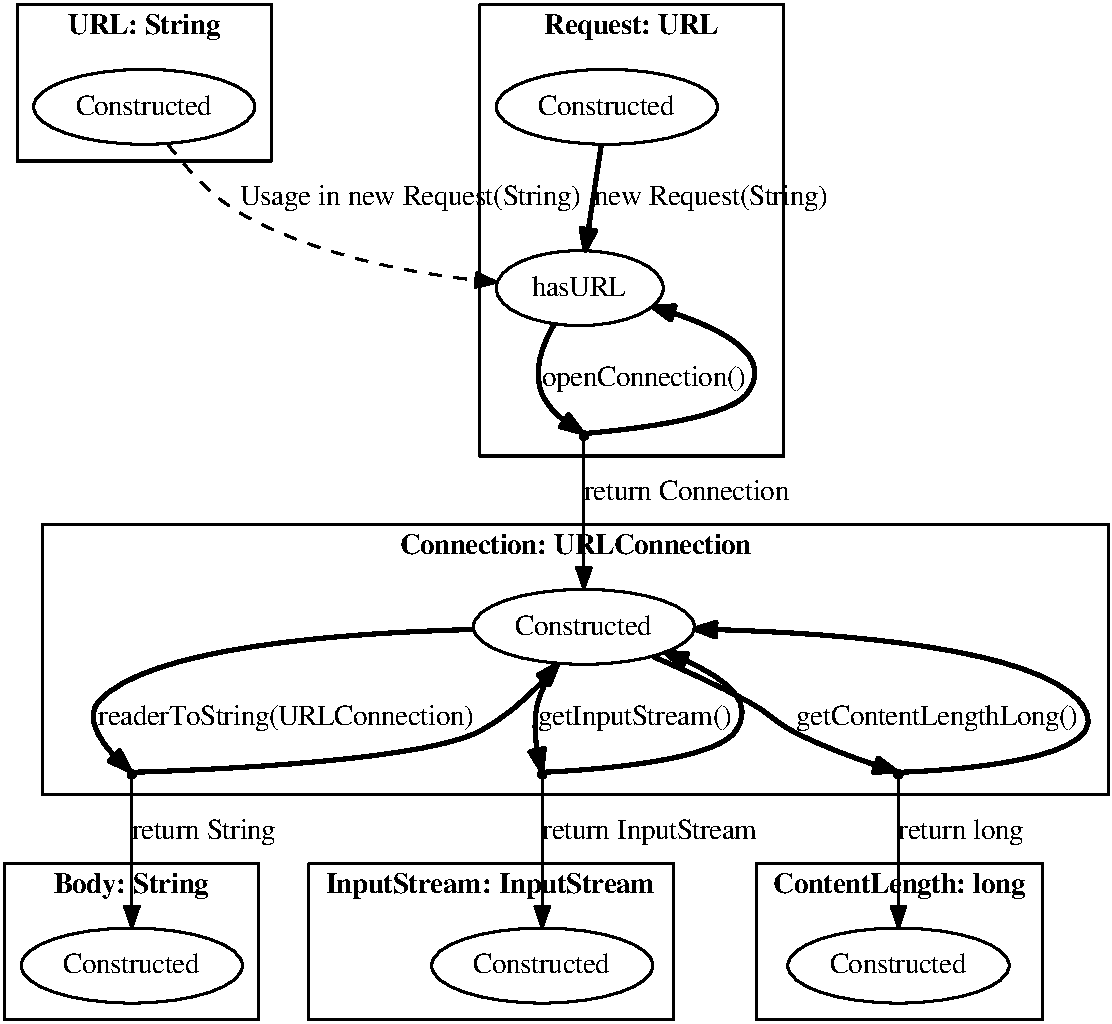
\includegraphics[width=0.75\textwidth]{java-cropped.pdf}
\end{center}
\end{frame}

{
\usebackgroundtemplate{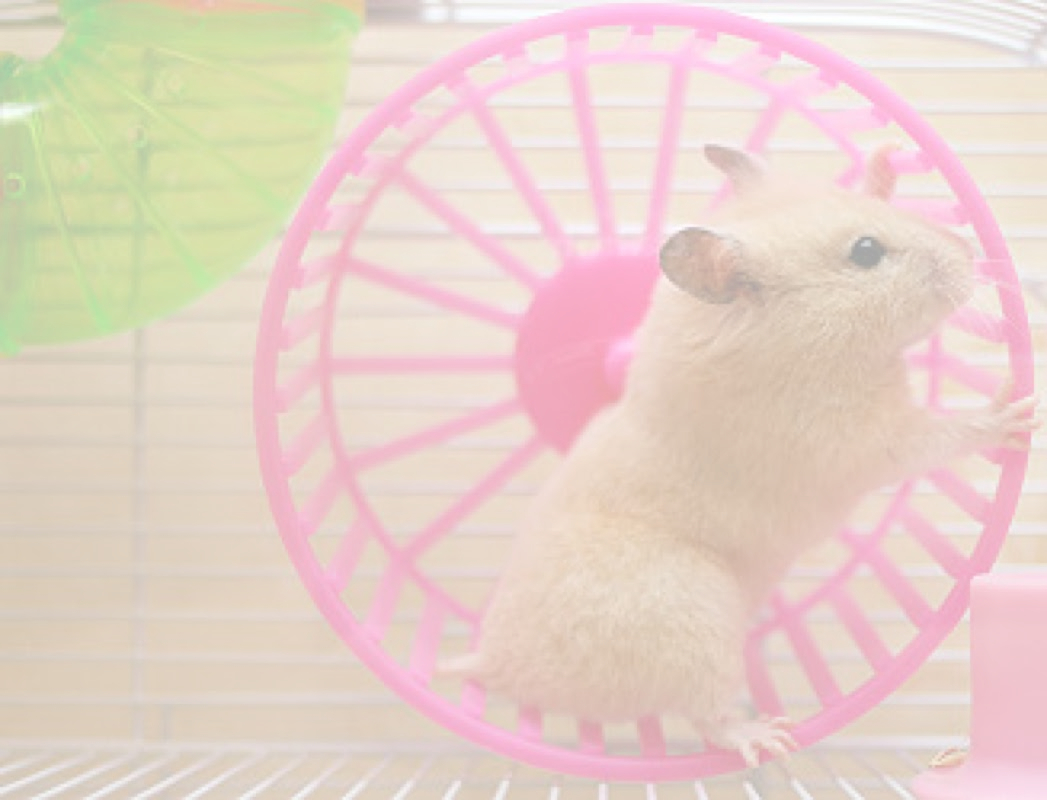
\includegraphics[height=\paperheight,width=\paperwidth]{wheel3.jpg};}
\begin{frame}{Что сделано}
  \begin{mybox}[]
  \begin{itemize}
  	\item Выбрана модель для описания библиотек
  	\item Сформирован DSL на Kotlin для описания моделей библиотек (частично)
  	\item Организовано портирование простых программ (искусственных и реальных)
  	\item Создана система проверки корректности преобразования
  \end{itemize}
  \end{mybox}
\end{frame}
}

{
\usebackgroundtemplate{
\includegraphics[height=\paperheight,width=\paperwidth]{todolist.jpg};}
\begin{frame}{Дальнейшее развитие}
	\begin{mybox}[]
	\begin{itemize}
		\item Расширение поддержки модели в прототипе
		\item Развитие метода поиска соответствия между автоматами
		\item Перепроектирование языка для описания моделей
		\item Пополнение репозитория моделей библиотек
		\item Проверка прототипа на более сложных тестовых программах
	\end{itemize}
	\end{mybox}
\end{frame}
}

\begin{frame}[t]{Контакты}
	Email: artyom.h31@gmail.com
	
	GitHub: \url{https://github.com/h31/LibraryMigration}
	
	\vspace{1cm}
	\begin{center}
		\Large
		Спасибо за внимание!
	\end{center}
\end{frame}

\begin{frame}[fragile]{Пример миграции. Программа <<До>>}

\begin{minted}[breaklines,fontsize=\footnotesize]{java}
URL url = new URL("http://api.ipify.org/");
URLConnection conn = url.openConnection();
if (conn.getContentLengthLong() > 0) {
    String response = new BufferedReader(new InputStreamReader(conn.getInputStream()))
    .lines().collect(Collectors.joining("\n"));
    System.out.println(response);
} else {
    System.out.println("Error!");
}
\end{minted}
\end{frame}

\begin{frame}[fragile]{Результат миграции. Программа <<После>>}
\begin{minted}[breaklines,fontsize=\scriptsize]{java}
HttpGet url = new HttpGet("http://api.ipify.org/");
CloseableHttpClient newMachine_Client_0 = HttpClients.createDefault();
CloseableHttpResponse conn = newMachine_Client_0.execute(url);
long linkedEdge_ContentLength_1 = conn.getEntity().getContentLength();
if (linkedEdge_ContentLength_1 > 0) {
    InputStream linkedEdge_InputStream_2 = conn.getEntity().getContent();
    String response = new BufferedReader(new InputStreamReader(linkedEdge_InputStream_2))
    .lines().collect(Collectors.joining("\n"));
    System.out.println(response);
} else {
    System.out.println("Error!");
}
\end{minted}
\end{frame}

\end{document}
